\documentclass{beamer}


\usetheme[progressbar=frametitle]{metropolis}
\usepackage{appendixnumberbeamer}

\usepackage{booktabs}
\usepackage[scale=2]{ccicons}

%\usepackage{pgfplots}
%\usepgfplotslibrary{dateplot}

\usepackage{xspace}
\newcommand{\themename}{\textbf{\textsc{metropolis}}\xspace}

%\setbeamertemplate{footline} % To remove the footer line in all slides uncomment this line
%\setbeamertemplate{footline}[page number] % To replace the footer line in all slides with a simple slide count uncomment this line

%\setbeamertemplate{navigation symbols}{} % To remove the navigation symbols from the bottom of all slides uncomment this line


\usepackage{graphicx} % Allows including images
\usepackage{grffile}
\usepackage{amsmath}
% have to have Mozilla's=Fira Sans} font and XeTeX installed to use full typography.

%----------------------------------------------------------------------------------------
%	TITLE PAGE
%----------------------------------------------------------------------------------------

\title{Alliance Treaty Design \\ and the Arms-Alliances Tradeoff}
\date{May 3, 2018}
\author{Joshua Alley}
\institute{Texas A\&M University}


\begin{document}

 \maketitle


%----------------------------------------------------------------------------------------
%	PRESENTATION SLIDES
%----------------------------------------------------------------------------------------

%------------------------------------------------
% This is my point. 
 \begin{frame}[standout]

Compared to alliances with no specific promises, unconditional alliance treaties decrease military spending.

 \end{frame}

%------------------------------------------------

 \begin{frame}{Why study the arms-alliances tradeoff: Part 1}

% put some sort of motivation, case/story/picture here. 

\only<1>{
\begin{figure}
	\centering
		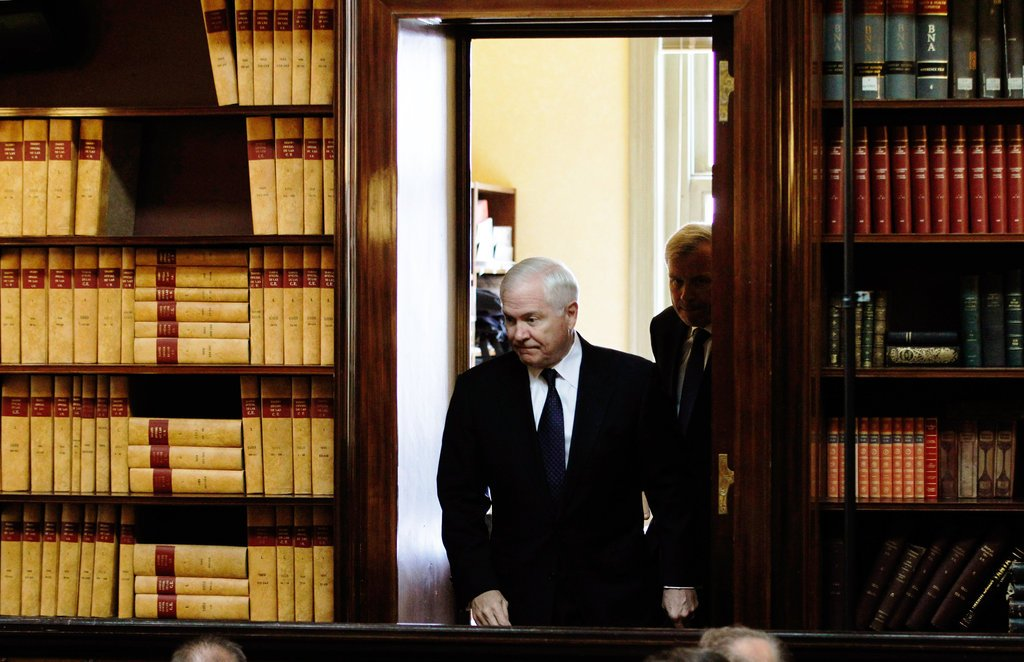
\includegraphics[width=0.95\textwidth]{gates-nato.jpg}
	\label{fig:gates-nato}
\end{figure}
}

\only<2>{``Nations apparently willing and eager for American taxpayers to assume the growing security burden left by reductions in European defense budgets.'' \emph{Robert Gates}}



 \end{frame}


%------------------------------------------------

\begin{frame}{Why study the arms-alliances tradeoff: Part 2}

Two theories predict states will substitute allied military spending for their own, but empirical evidence is mixed:

\pause

\begin{tabular}{lc}
Paper & Finding \\
\hline
Conybeare 1992 & --  \\
Morrow 1993 & -- \\
\pause 
Diehl 1994 & + \\
Morgan and Palmer 2006 & + \\ 
\pause 
Quiroz-Flores 2011 & + \\ 
Pl{\"u}mper and Neumayer 2015 & -- \\
\pause 
DiGiuseppe and Poast 2016 & -- \\ 
Horowitz et al 2017 & + \\ 

\end{tabular}




 \end{frame}


%------------------------------------------------

\begin{frame}{Outline}

I argue that unconditional treaties are more likely to lead to substitution in two ways: 

\pause

\begin{enumerate}
\item Theory
\pause
\item Statistical Analysis
\end{enumerate}




 \end{frame}

%------------------------------------------------

\section{Theory}

%------------------------------------------------

\begin{frame}{Substitution}

\pause

Arms and alliances are imperfect substitutes: 
\pause 
\begin{enumerate}
\item Arms are a reliable source of capability, but develop slowly. 
\pause 
\item Alliances are less reliable than arms, but offer immediate capability gains. 
\end{enumerate} 
\pause 

\end{frame}

%------------------------------------------------
 
\begin{frame}[standout]

More reliable alliances are a better substitute for domestic arms. 

\end{frame}


%------------------------------------------------

\begin{frame}{Treaty Design and Alliance Reliability}

\pause

Alliance Capability Gains $=$ Pr(Support) * Value of Support:

\pause

\begin{enumerate}

\item Fewer conditions for intervention $\uparrow$ Pr(Support)

\pause

\item Promises to fight $\uparrow$ Value 


\end{enumerate} 


\end{frame}

%------------------------------------------------

\begin{frame}{Classifying Alliances}

Benson (2012) provides a typology of alliances:



\begin{itemize}

\pause

\item \textit{Unconditional Alliances} promise military support regardless of how a conflict began. 

\pause

\item \textit{Conditional Alliances} promise military support if particular conditions are met. 

\pause

\item \textit{Probabilistic Deterrent Alliances} do not guarantee military support or intervention.

\end{itemize}


\end{frame}

%------------------------------------------------

\begin{frame}{Prediction}

% Only do one here in the interest of time. 

\pause

\begin{quote}
\textsc{Hypothesis}: Unconditional alliances will be associated with decreases in defense spending by member states. 
\end{quote} 



\end{frame}

%------------------------------------------------

\section{Empirical Analysis} 

%-----------------------------------------------

\begin{frame}{Research Design: Multilevel Model}

\pause
Political Science Examples: Steenbergen and Jones 2002, Gelman and Hill 2007, Hee Park and Jensen 2007, Rainey 2015

\pause
Advantages: 
\begin{itemize}
\item Direct test of theory
\pause
\item Retain alliance-level variation
\pause 
\item Partial pooling for alliance comparisons
\end{itemize}

\end{frame}

%------------------------------------------------
 
\begin{frame}{Multilevel \& Multiple Membership Model}

\begin{equation*} 
y_{it} \sim student_t(\nu, \mu, \sigma) 
\end{equation*}

\begin{equation*}
\mu_{it} = \alpha + \alpha^{st} + \alpha^{yr} + \eta y_{it-1} + W_{it} \gamma + Z_{it} \lambda
\end{equation*}

\begin{equation*}
\lambda_k \sim N(\theta_k , \sigma^{all})
\end{equation*} 

\begin{equation*}
\theta = X \beta
\end{equation*}

\end{frame}

%------------------------------------------------
 
\begin{frame}{Empirical Model: Multilevel \& Multiple Membership}
 
\setbeamercovered{transparent}

\begin{equation*} 
y_{it} \sim student_t(\nu, \mu, \sigma) 
\end{equation*}

\pause

\begin{equation*}
\uncover<2->{\mu_{it} =} \uncover<3>{\alpha} \uncover<4>{+ \alpha^{st} + \alpha^{yr}} \uncover<5>{+ \eta y_{it-1}} \uncover<6>{+ W_{it} \gamma} \uncover<7>{+ Z_{it} \lambda}
\end{equation*}

Example year: 

\begin{equation*}
\begin{split}
& \uncover<2->{\mbox{Argentina 1955} = } \uncover<3>{\mbox{Overall mean}} \\
& \uncover<4>{+ \mbox{Argentine Intercept} + \mbox{1955 Intercept}} \\
& \uncover<5>{+ \mbox{1954 Spending}} \uncover<6>{+ \mbox{Argentine Characteristics}} \\
& \uncover<7>{+ \lambda_{OAS} * \mbox{OAS Expenditure} + \lambda_{Rio} * \mbox{Rio Pact Expenditure}}
\end{split}
\end{equation*}



\end{frame}

%------------------------------------------------

\begin{frame}[standout]{Z} 

\begin{tabular}{lccc}
State-Year & Rio Pact & Warsaw Pact & \ldots \\
\hline
Argentina 1954 & .347 & 0 & \ldots \\
Argentina 1955 & .418  & 0 & \ldots  \\
 \vdots & \vdots & \vdots & \ldots  
\end{tabular}

 \end{frame}

%------------------------------------------------

 
\begin{frame}{Predicting Alliance Weights $\lambda$}
 
\setbeamercovered{transparent}

\begin{equation*}
\lambda_k \sim N(\theta_k , \sigma^{all})
\end{equation*} 

\pause

\begin{equation*}
\theta = X \beta
\end{equation*}

\pause 

Example:

\begin{equation*}
\lambda_{Rio} = \beta_1 + \beta_2 \mbox{Unconditional} + \beta_3 \mbox{Conditional} + \beta_4 \mbox{Prob. Det.} + \mbox{Controls}
\end{equation*}


\end{frame}

%------------------------------------------------

\begin{frame}{Sample and Key Variables}

\begin{itemize}
\item \textbf{Sample}: 159 non-major powers and 314 alliances, 1950-2001. 
\pause 
\item \textbf{DV}: Ln(Military Spending) 
\pause
\item \textbf{Key Alliance Variables}: Binary indicators of Unconditional, Conditional, and Probabilistic Deterrent conditions. 
\pause
\item \textbf{Base Category}: Consultation/Non-aggression Pacts (179 alliances)
\pause
\item \textbf{Alliance Controls}: Institutionalization, Compellent Aims, Military Aid, Proportion of Democratic Members, Wartime, US member, Russia Member
\pause
\item \textbf{State-level Controls}: Interstate war, Civil War, GDP, POLITY, Cold War, Rival military expenditures

\end{itemize} 



\end{frame}

%------------------------------------------------

\section{Results}

%------------------------------------------------

\begin{frame}{Posterior of Unconditional Coefficient} 


\begin{figure}
	\centering
		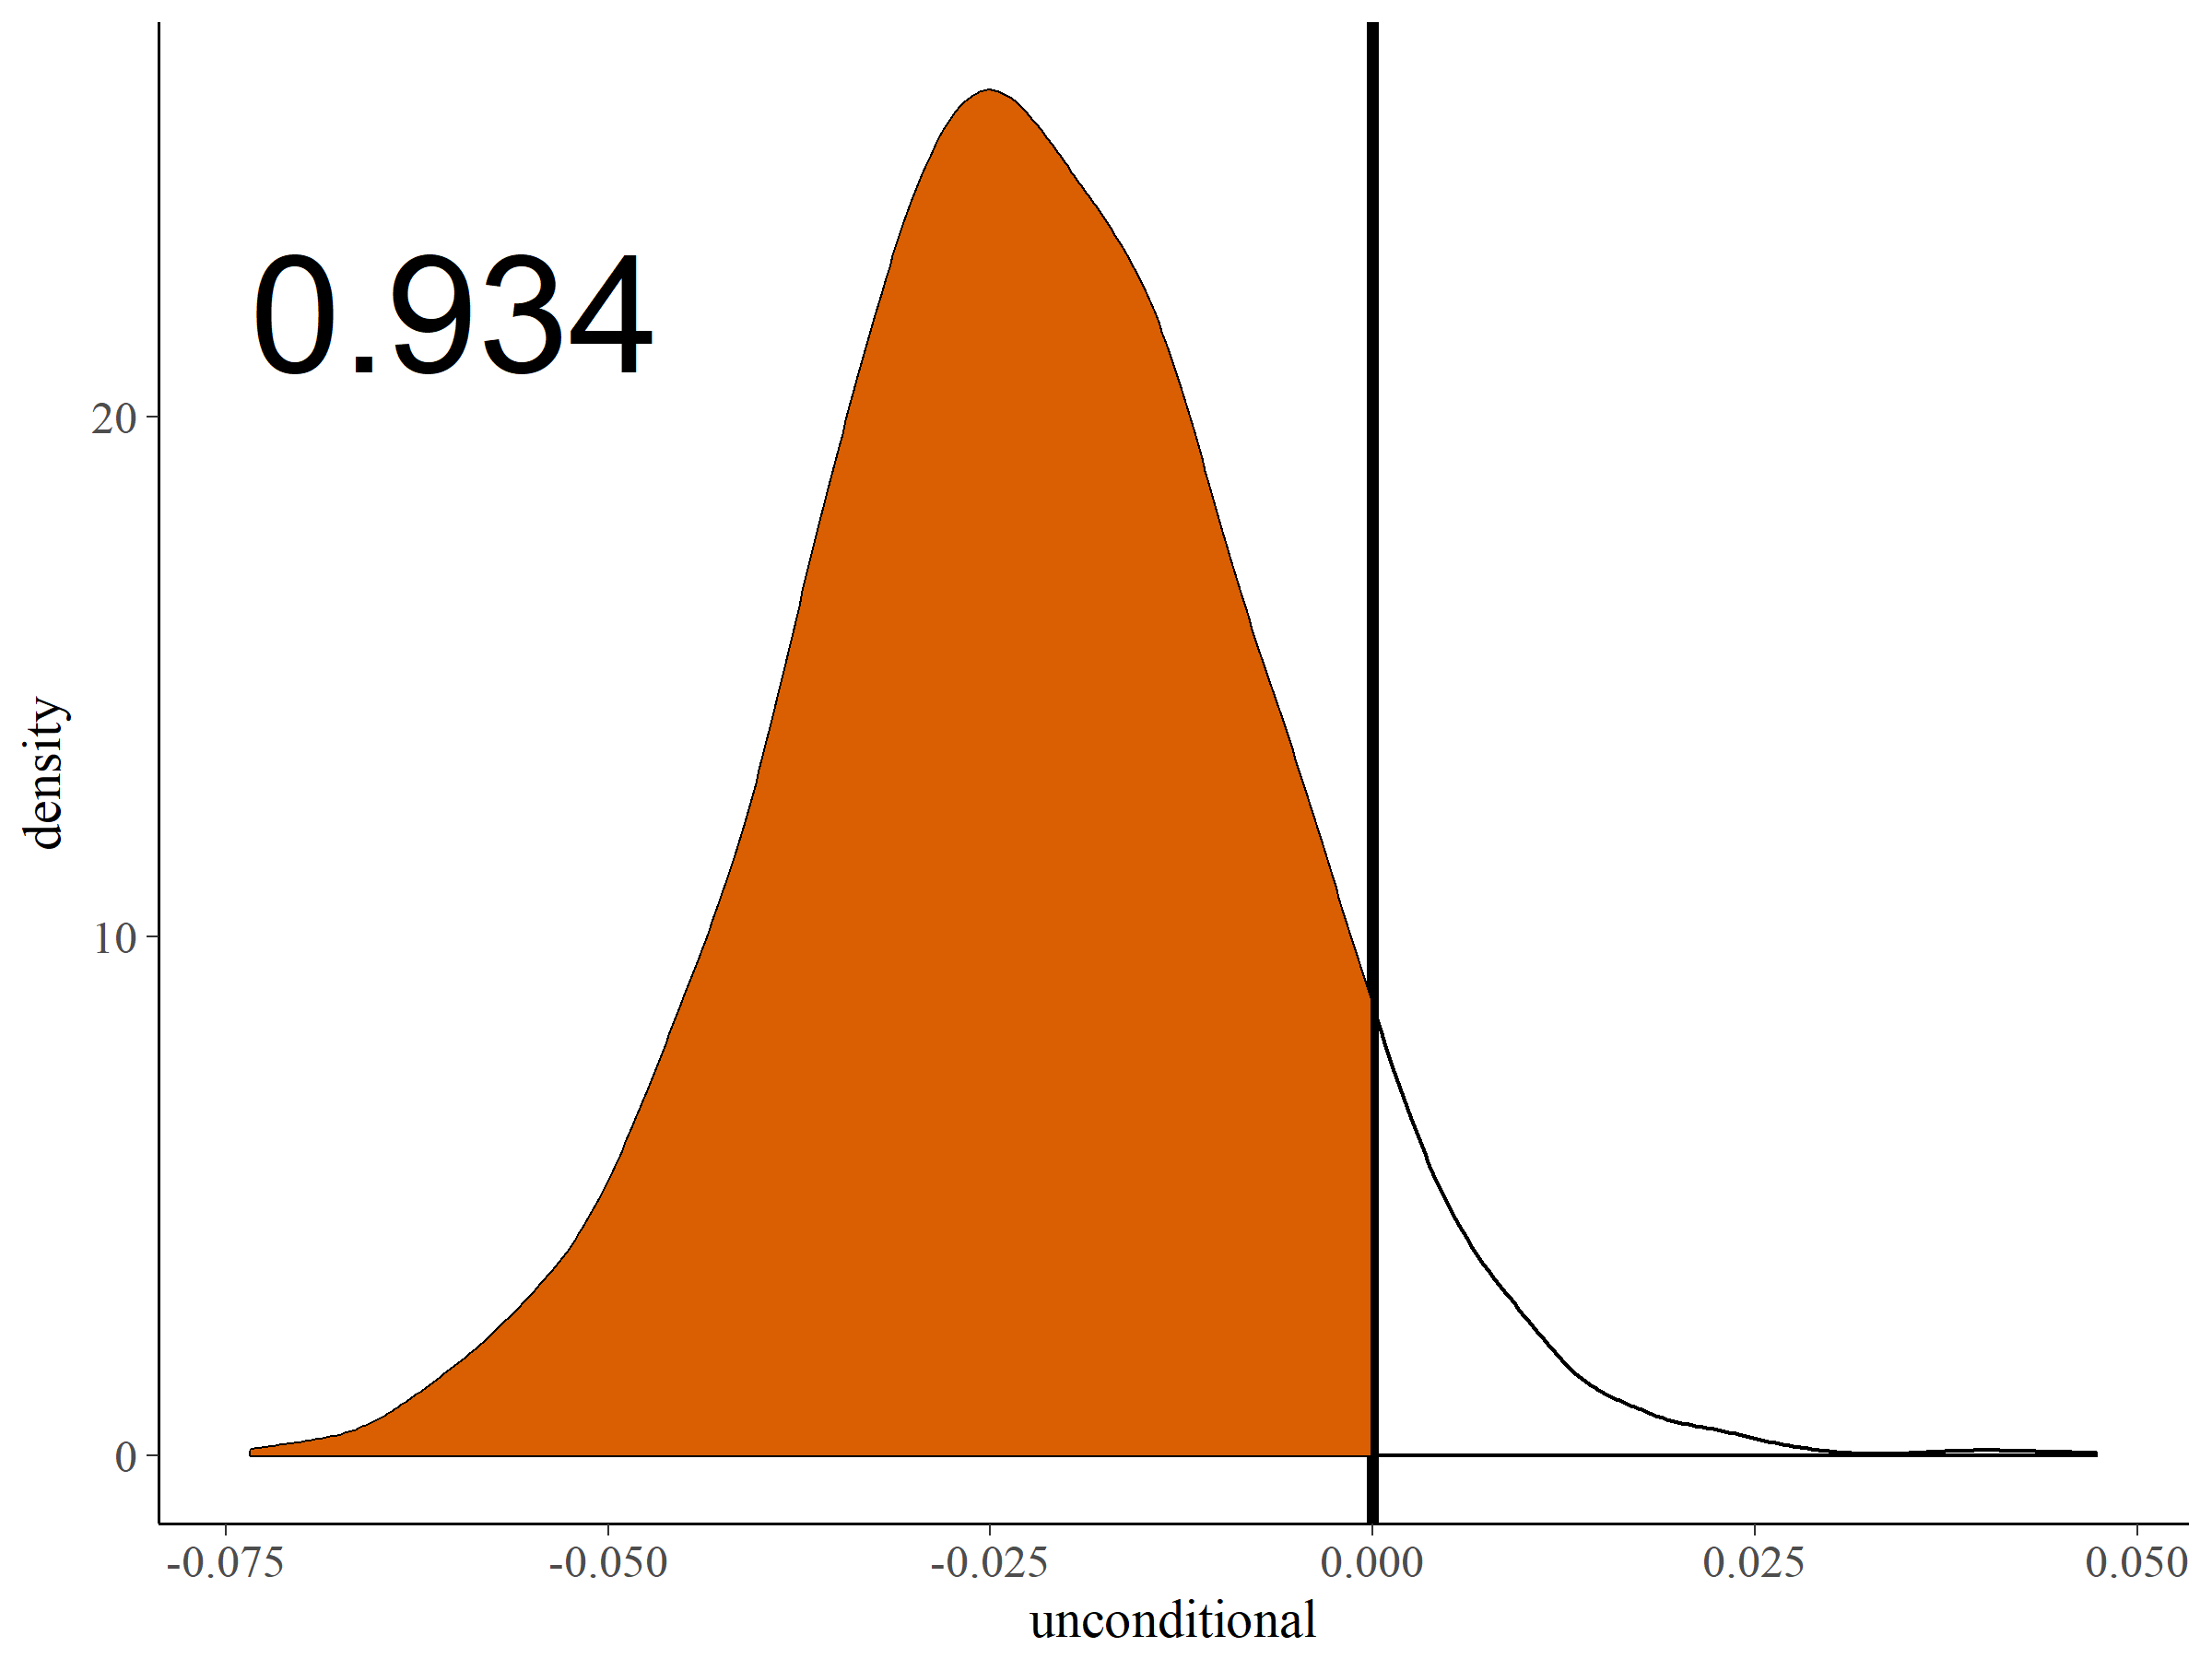
\includegraphics[width=0.95\textwidth]{uncond post_prob.png}
	\label{fig:uncond post_prob}
\end{figure}



\end{frame}

%------------------------------------------------

\begin{frame}[standout]{Long Run Multiplier} 

\begin{tabular}{lcc}
Variable & Posterior Mean & $Pr(X < 0)$ \\
\hline
Unconditional & -0.75 & .934 \\
\pause
POLITY & -0.68 & .99  \\
\end{tabular}

 \end{frame}




%-----------------------------------------------

\begin{frame}{Violin Plot of Weight Parameters}

\begin{figure}
	\centering
		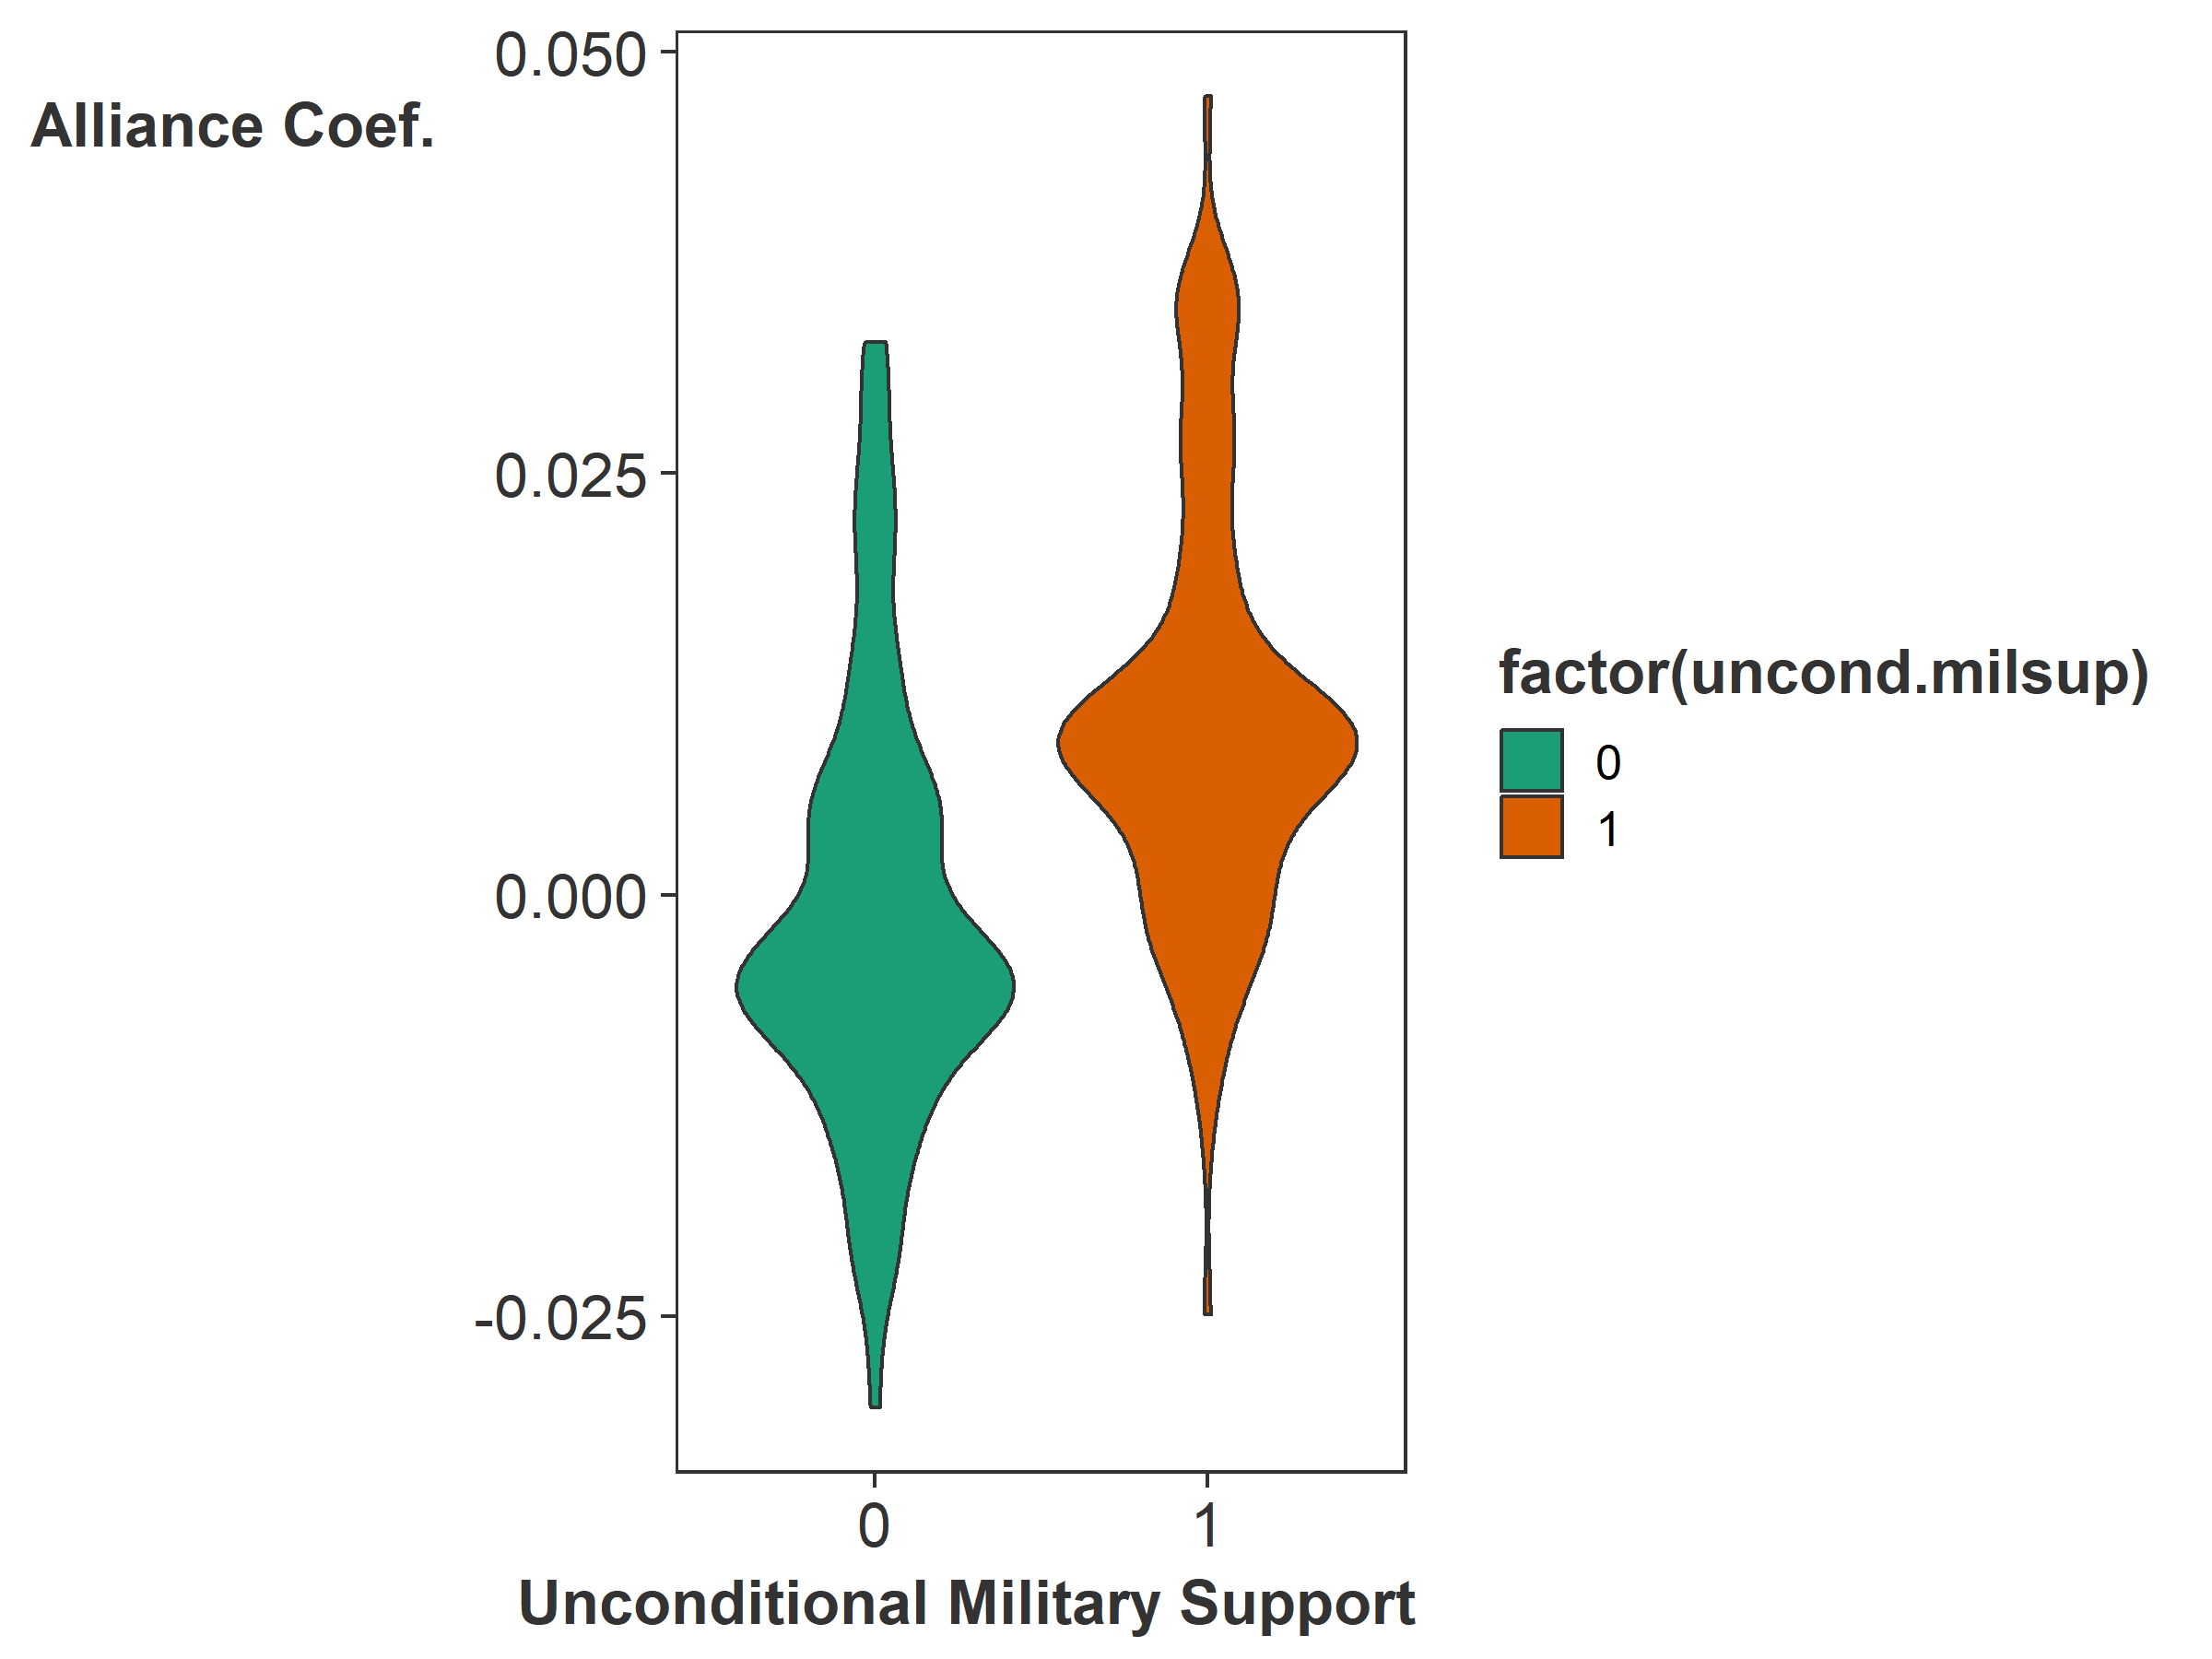
\includegraphics[width=0.95\textwidth]{lambda-box-presentation.png}
	\label{fig:lambdac none-uncond}
\end{figure}


\end{frame}



%-----------------------------------------------

\section{Discussion and Conclusion}

%-----------------------------------------------

\begin{frame}{Discussion}

\pause 
Limitations:
\pause
\begin{enumerate}
\item My theory does not address cases where arms and allies are complements. 
\pause
\item Strategic Alliance Design: addressed through controls
\pause 
\item No time-varying alliance characteristics
\end{enumerate}

\end{frame}


%-----------------------------------------------

\begin{frame}{Conclusion}

Compared to alliances with no specific promises, unconditional alliance treaties decrease military spending.

\pause

Implications and Extensions:
\pause
\begin{itemize}
\item Arms and allies as complements
\pause
\item Domestic arms development and substitution
\pause
\item Political economy of international security
\end{itemize}

\end{frame}


%-----------------------------------------------

\appendix 

%------------------------------------------------


\begin{frame}{Trace Plots for $\beta$}

\begin{figure}
	\centering
		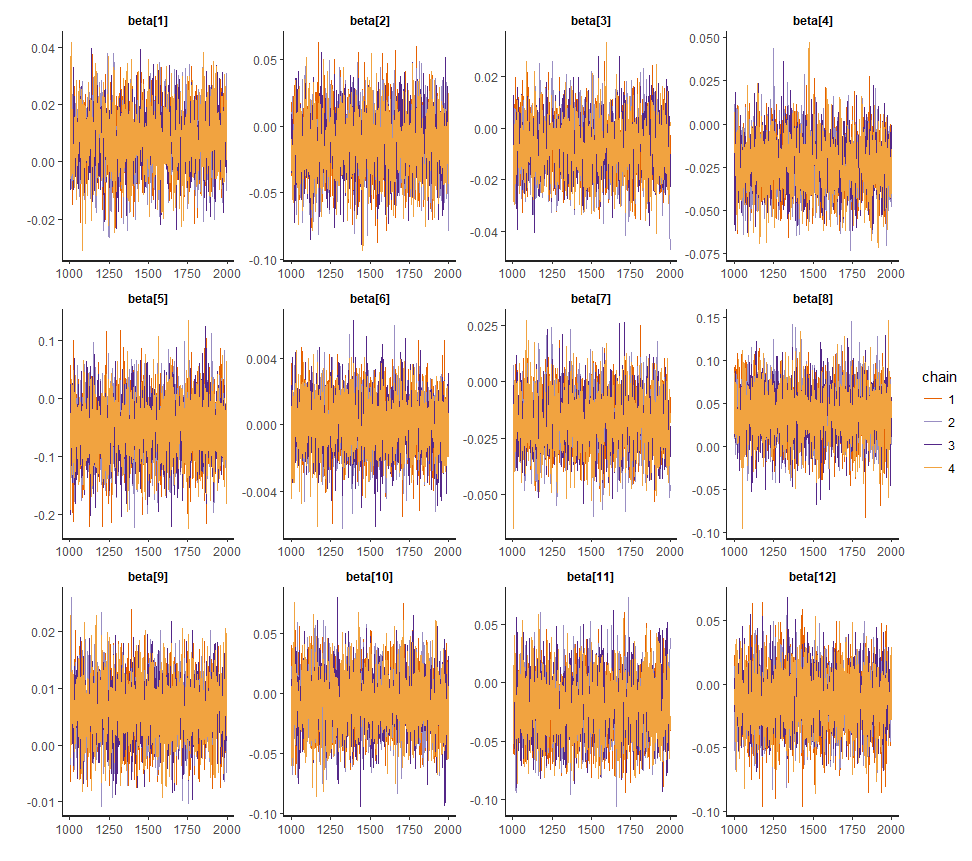
\includegraphics[width=0.85\textwidth]{beta trace.png}
	\label{fig:beta trace}
\end{figure}


\end{frame}

%-----------------------------------------------

\begin{frame}{Posterior Predictive Check}


\begin{figure}
	\centering
		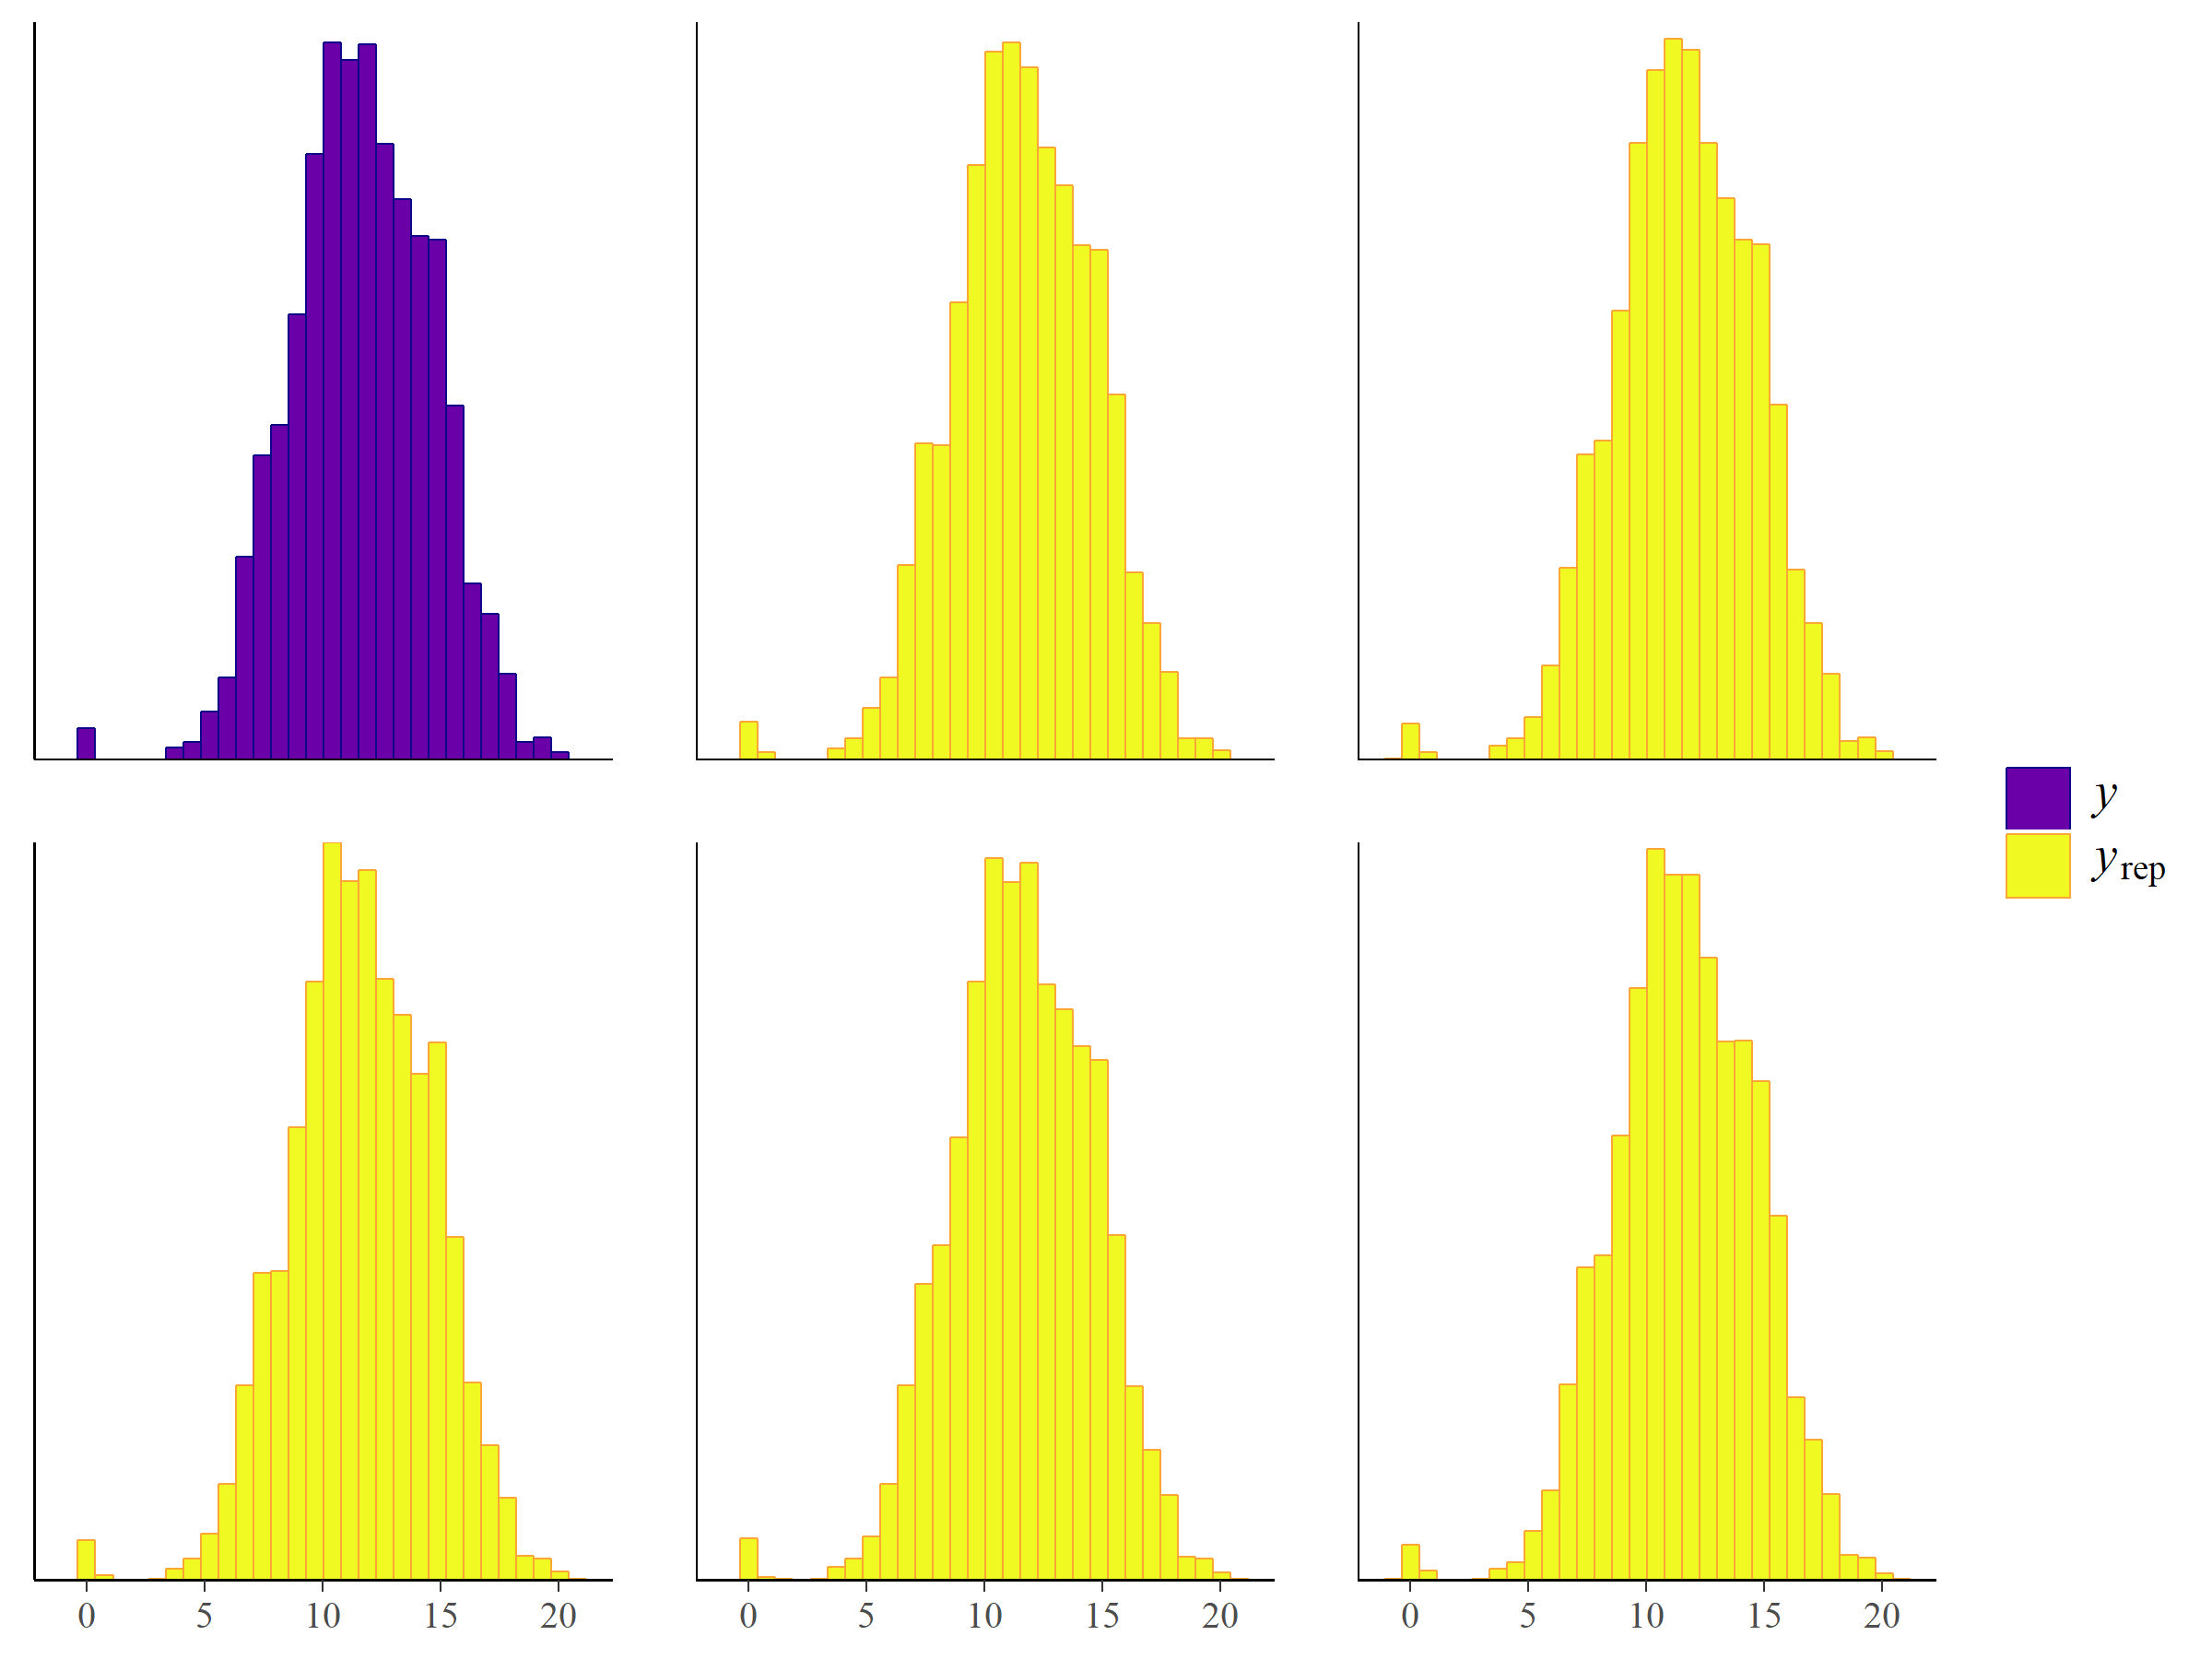
\includegraphics[width=0.95\textwidth]{ppc.png}
	\label{fig:ppc}
\end{figure}


\end{frame}


%------------------------------------------------


\begin{frame}{Priors}

\begin{table} % Create a table of priors.

 \begin{center}
\begin{tabular}{c} 
$ p(\alpha) \sim N(0, 3)$  \\
$ p(\sigma) \sim \mbox{half-}N(0, 1) $ \\
$ p(\alpha^{yr}) \sim N(0, \sigma^{yr}) $ \\ 
$ p(\sigma^{yr}) \sim N(0, 1) $ \\
$ p(\alpha^{st}) \sim N(0, \sigma^{st}) $ \\ 
$ p(\sigma^{st}) \sim \mbox{half-}N(0, 1) $ \\ 
$ p(\sigma^{all}) \sim \mbox{half-}N(0, 1) $ \\
$ p(\eta) \sim \mbox{half-}N(0, 1) $ \\
$ p(\beta) \sim N(0, 1) $ \\
$ p(\gamma) \sim N(0, 1) $ \\ 
$ p(\nu) \sim gamma(2, 0.1)$ 
\end{tabular} 
\end{center} 
\label{tab:priors}
\end{table} 


\end{frame}

%------------------------------------------------

\begin{frame}{Positive Posterior Probability of all Coefficients}

\begin{figure}
	\centering
		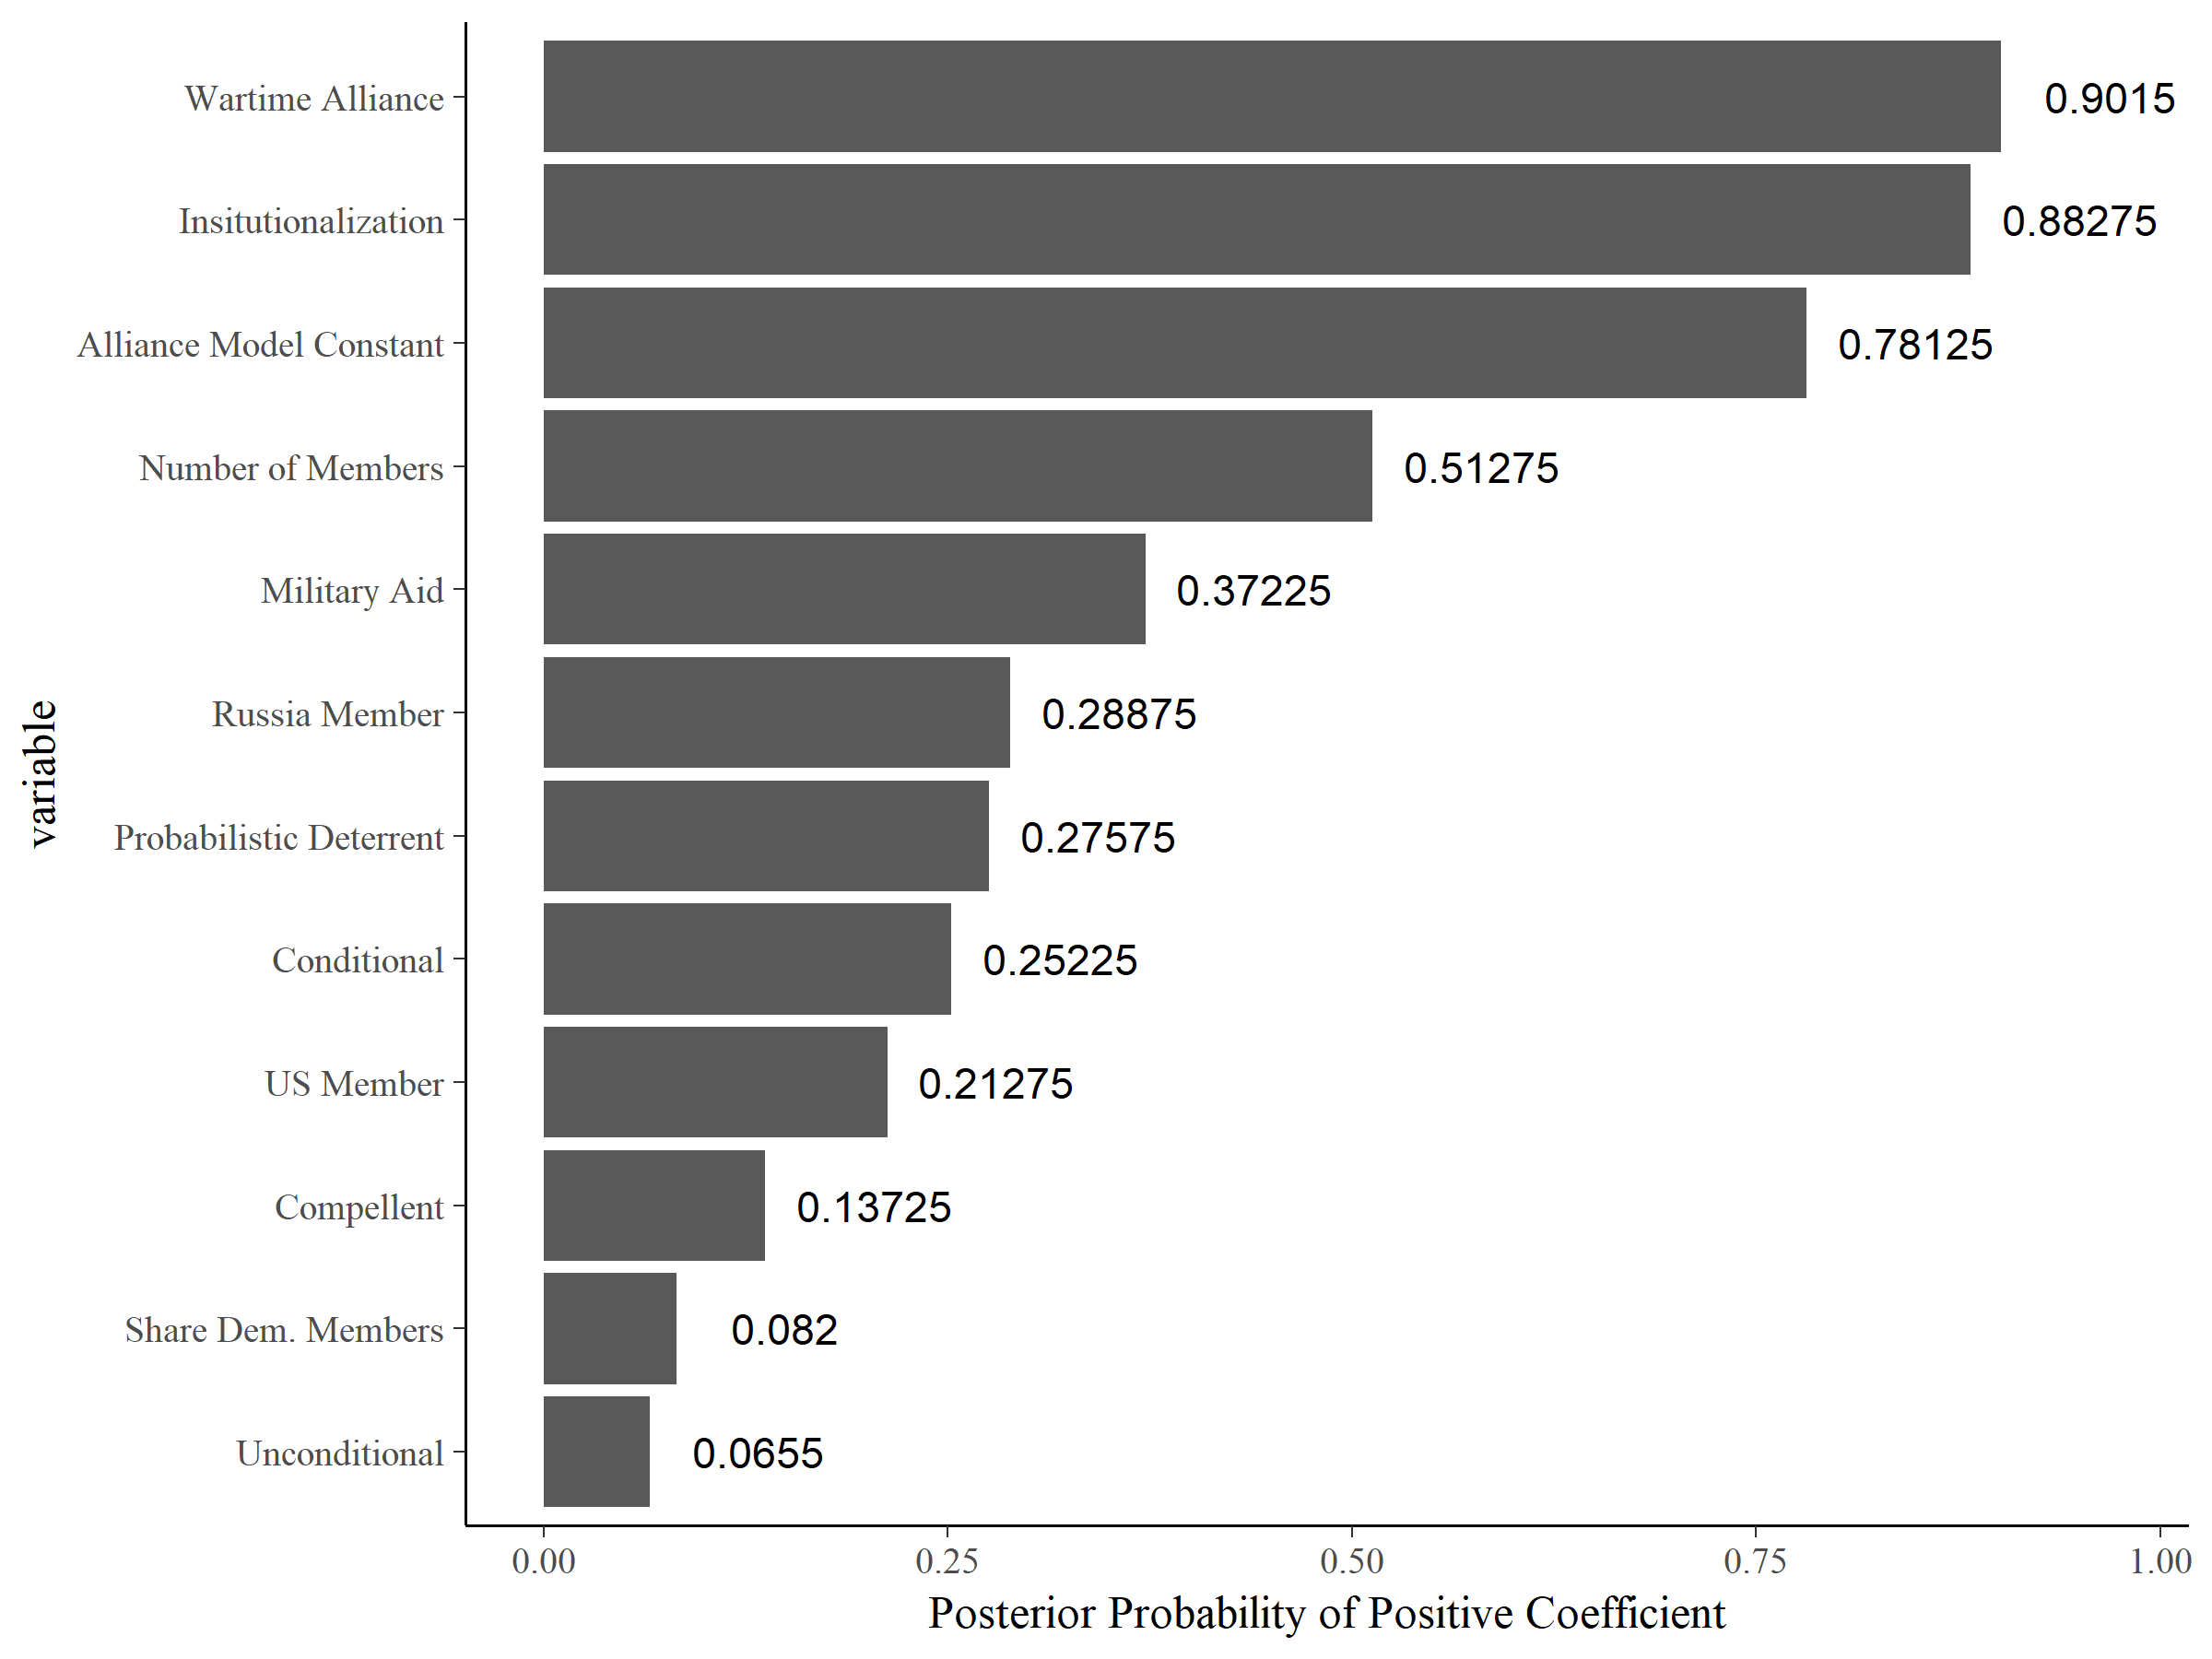
\includegraphics[width=0.95\textwidth]{post-prob-beta.png}
	\label{fig:post-prob-beta}
\end{figure}


\end{frame}

%------------------------------------------------

\begin{frame}{90\% Credible Intervals for Alliance Covariates}


\begin{table}[ht]
\centering
\begin{tabular}{rrrrrr}
  \hline
 & mean & sd & 5\% & 95\% & n\_eff  \\ 
  \hline
Constant & 0.008 & 0.010 & -0.009 & 0.025 & 2503.930  \\ 
  Prob. Det. & -0.013 & 0.023 & -0.051 & 0.023 & 4000.000  \\ 
  Conditional & -0.007 & 0.011 & -0.025 & 0.011 & 2278.851 \\ 
  \textbf{Uncond. Det.} & -0.023 & 0.015 & -0.048 & 0.002 & 3009.267  \\ 
  Compellent & -0.054 & 0.050 & -0.137 & 0.031 & 4000.000  \\ 
  Num. Members & 0.000 & 0.002 & -0.003 & 0.003 & 4000.000  \\ 
  Dem. Share & -0.018 & 0.012 & -0.037 & 0.003 & 2618.817 \\ 
  Wartime & 0.038 & 0.030 & -0.011 & 0.087 & 4000.000  \\ 
  Institutionalization & 0.006 & 0.005 & -0.002 & 0.015 & 4000.000  \\ 
  Military aid & -0.008 & 0.024 & -0.046 & 0.033 & 4000.000  \\ 
  US Member & -0.020 & 0.025 & -0.062 & 0.021 & 3091.589 \\ 
  Russia Member & -0.013 & 0.022 & -0.050 & 0.024 & 4000.000  \\ 
   \hline
\end{tabular}
\end{table}

\end{frame}


%------------------------------------------------

\begin{frame}{90\% Credible Intervals for State Covariates}

\begin{table}[ht]
\centering
\begin{tabular}{rrrrrr}
  \hline
    & mean & sd & 5\% & 95\% & n\_eff  \\ 
  \hline
	Lagged Expenditures & 0.97 & 0.00 & 0.96 & 0.98 & 747.65  \\ 
  Wartime & 0.07 & 0.01 & 0.04 & 0.09 & 4000.00 \\ 
  Civil War & 0.04 & 0.01 & 0.02 & 0.06 & 4000.00  \\ 
  Rival Mil. Expenditure & -0.01 & 0.01 & -0.02 & 0.00 & 4000.00  \\ 
  ln(GDP) & 0.11 & 0.02 & 0.09 & 0.14 & 830.46   \\ 
  Polity & -0.02 & 0.01 & -0.03 & -0.01 & 4000.00 \\ 
  Cold War & 0.04 & 0.01 & 0.02 & 0.06 & 1292.56  \\ 
  $\sigma$ State & 0.02 & 0.01 & 0.01 & 0.03 & 486.70  \\ 
  $\alpha$ & 0.20 & 0.03 & 0.14 & 0.26 & 789.97  \\ 
   \hline
\end{tabular}
\end{table}


\end{frame}

%------------------------------------------------

\begin{frame}{Posterior of Probabilistic Deterrent Coefficient}

\begin{figure}
	\centering
		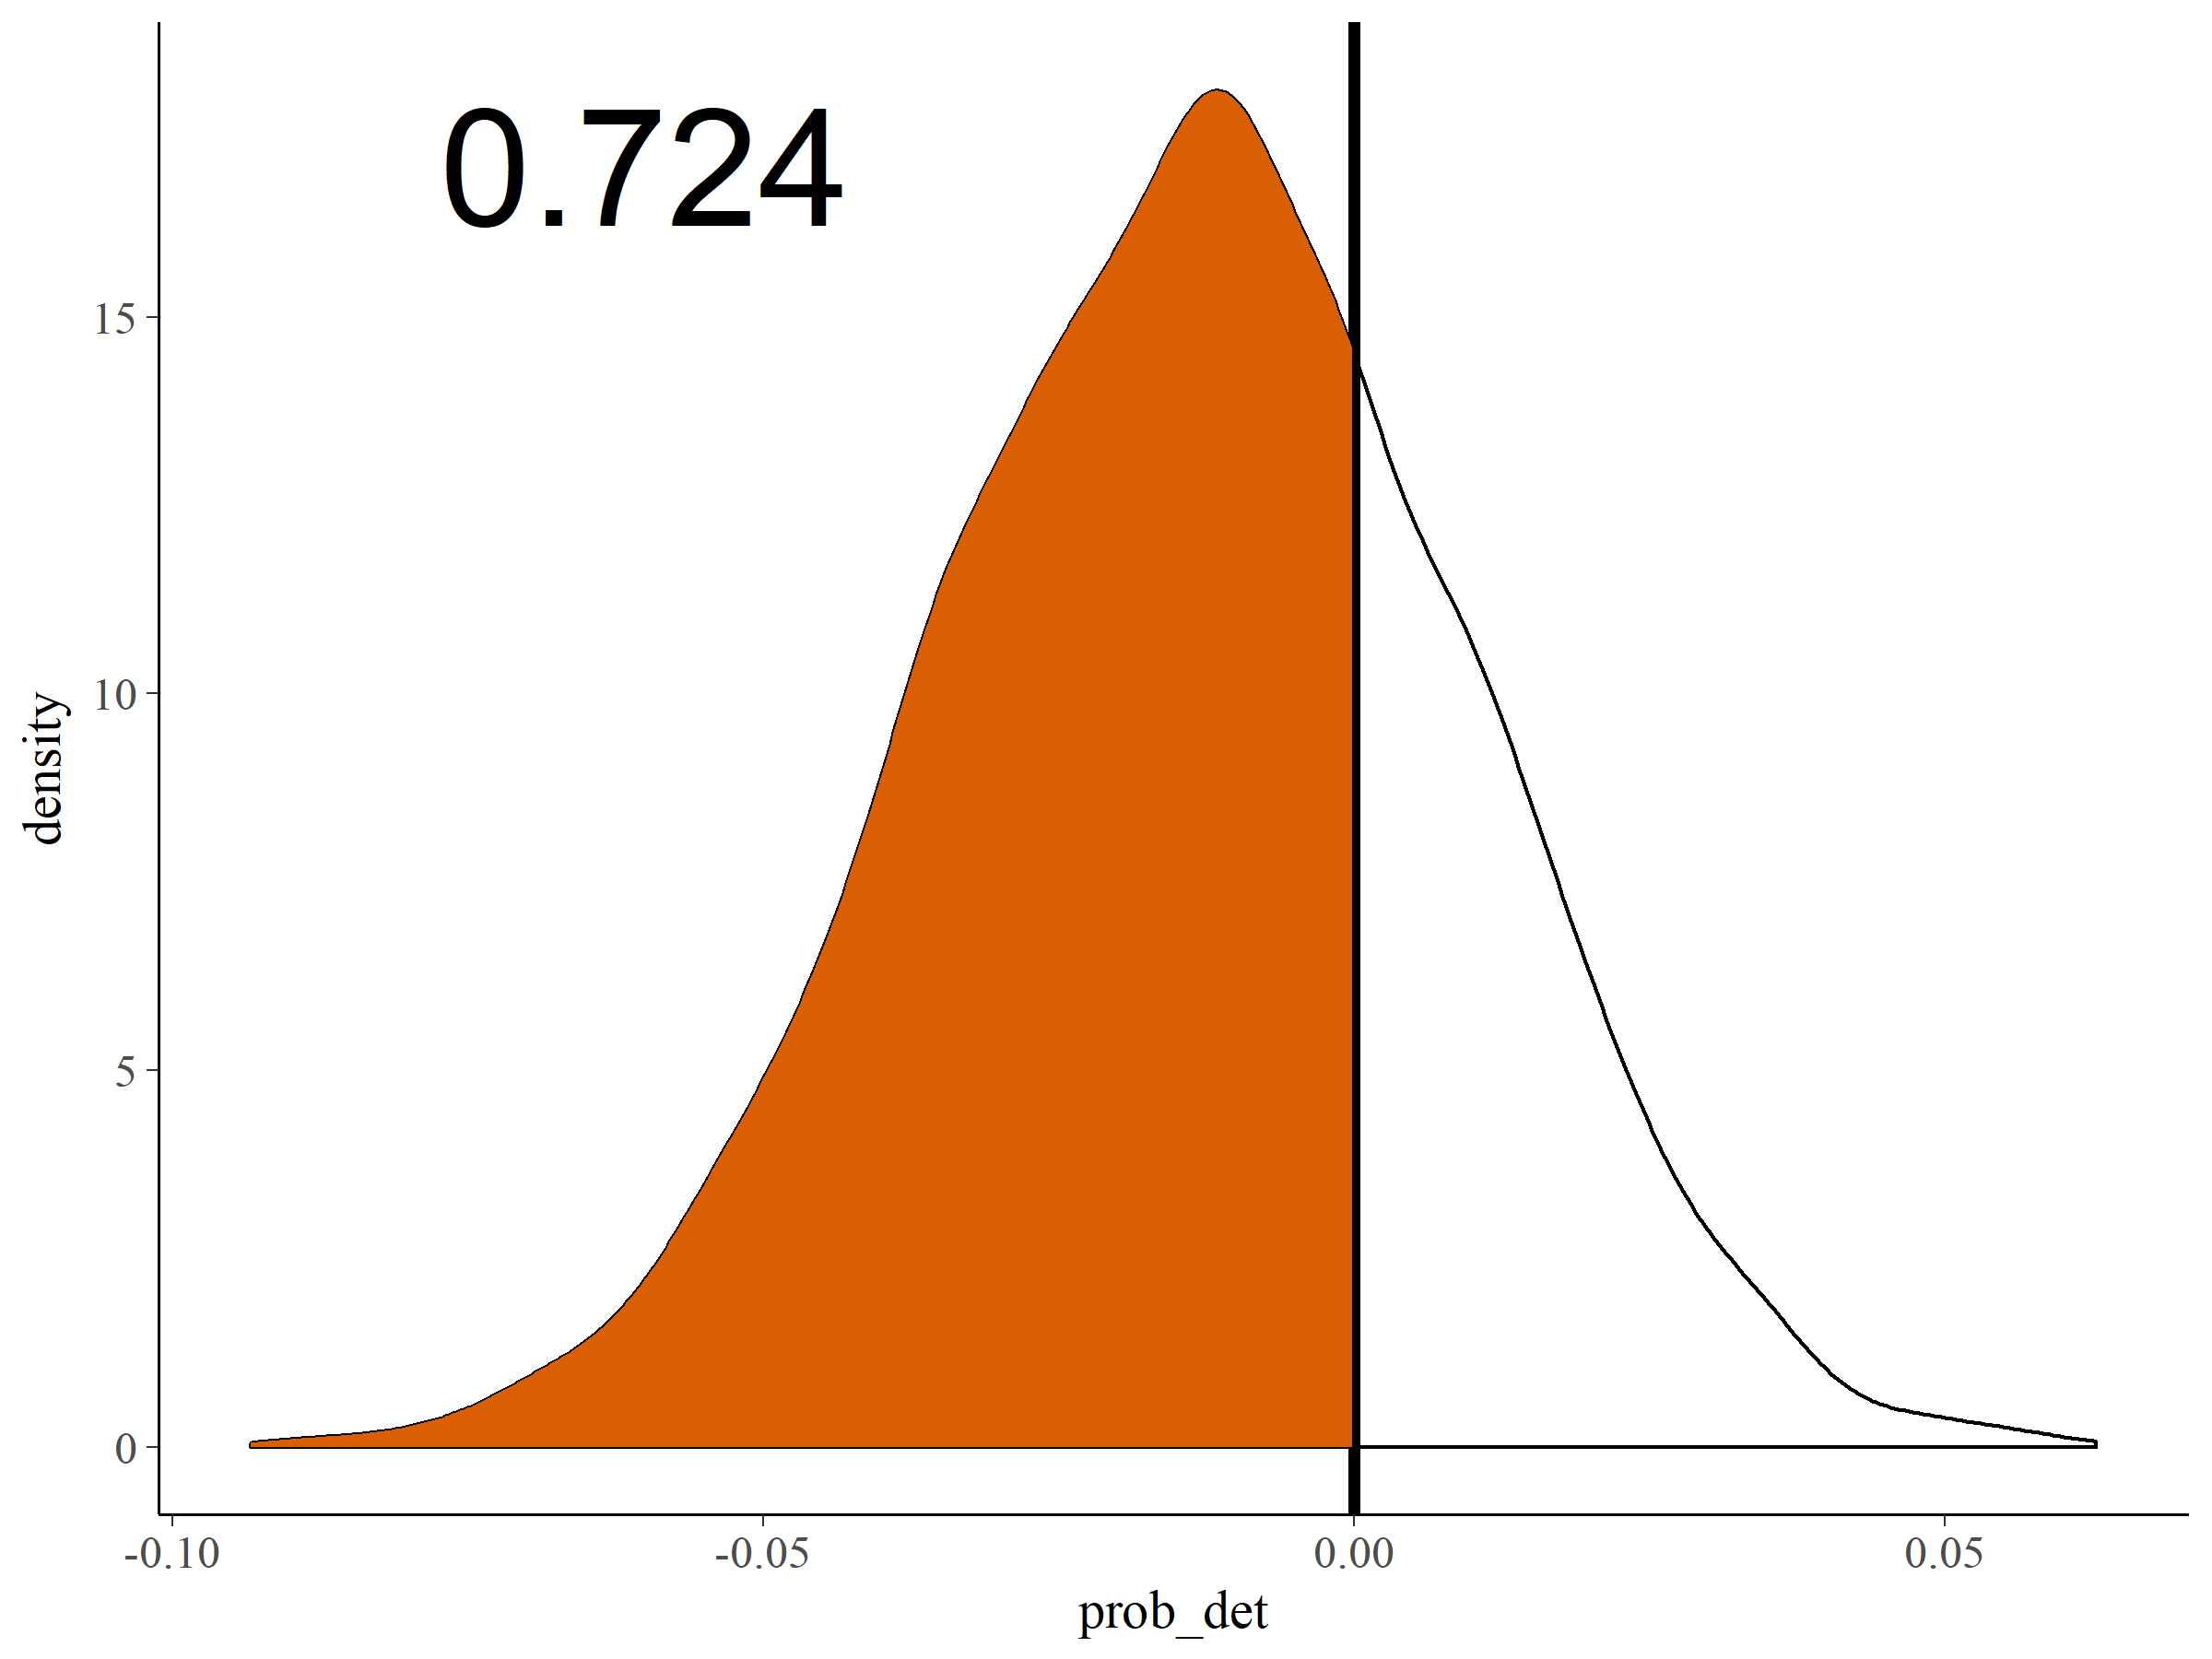
\includegraphics[width=0.95\textwidth]{probdet post_prob.png}
	\label{fig:probdet post_prob}
\end{figure}


\end{frame}

%------------------------------------------------

\begin{frame}{Non-zero alliances}

\begin{figure}
	\centering
		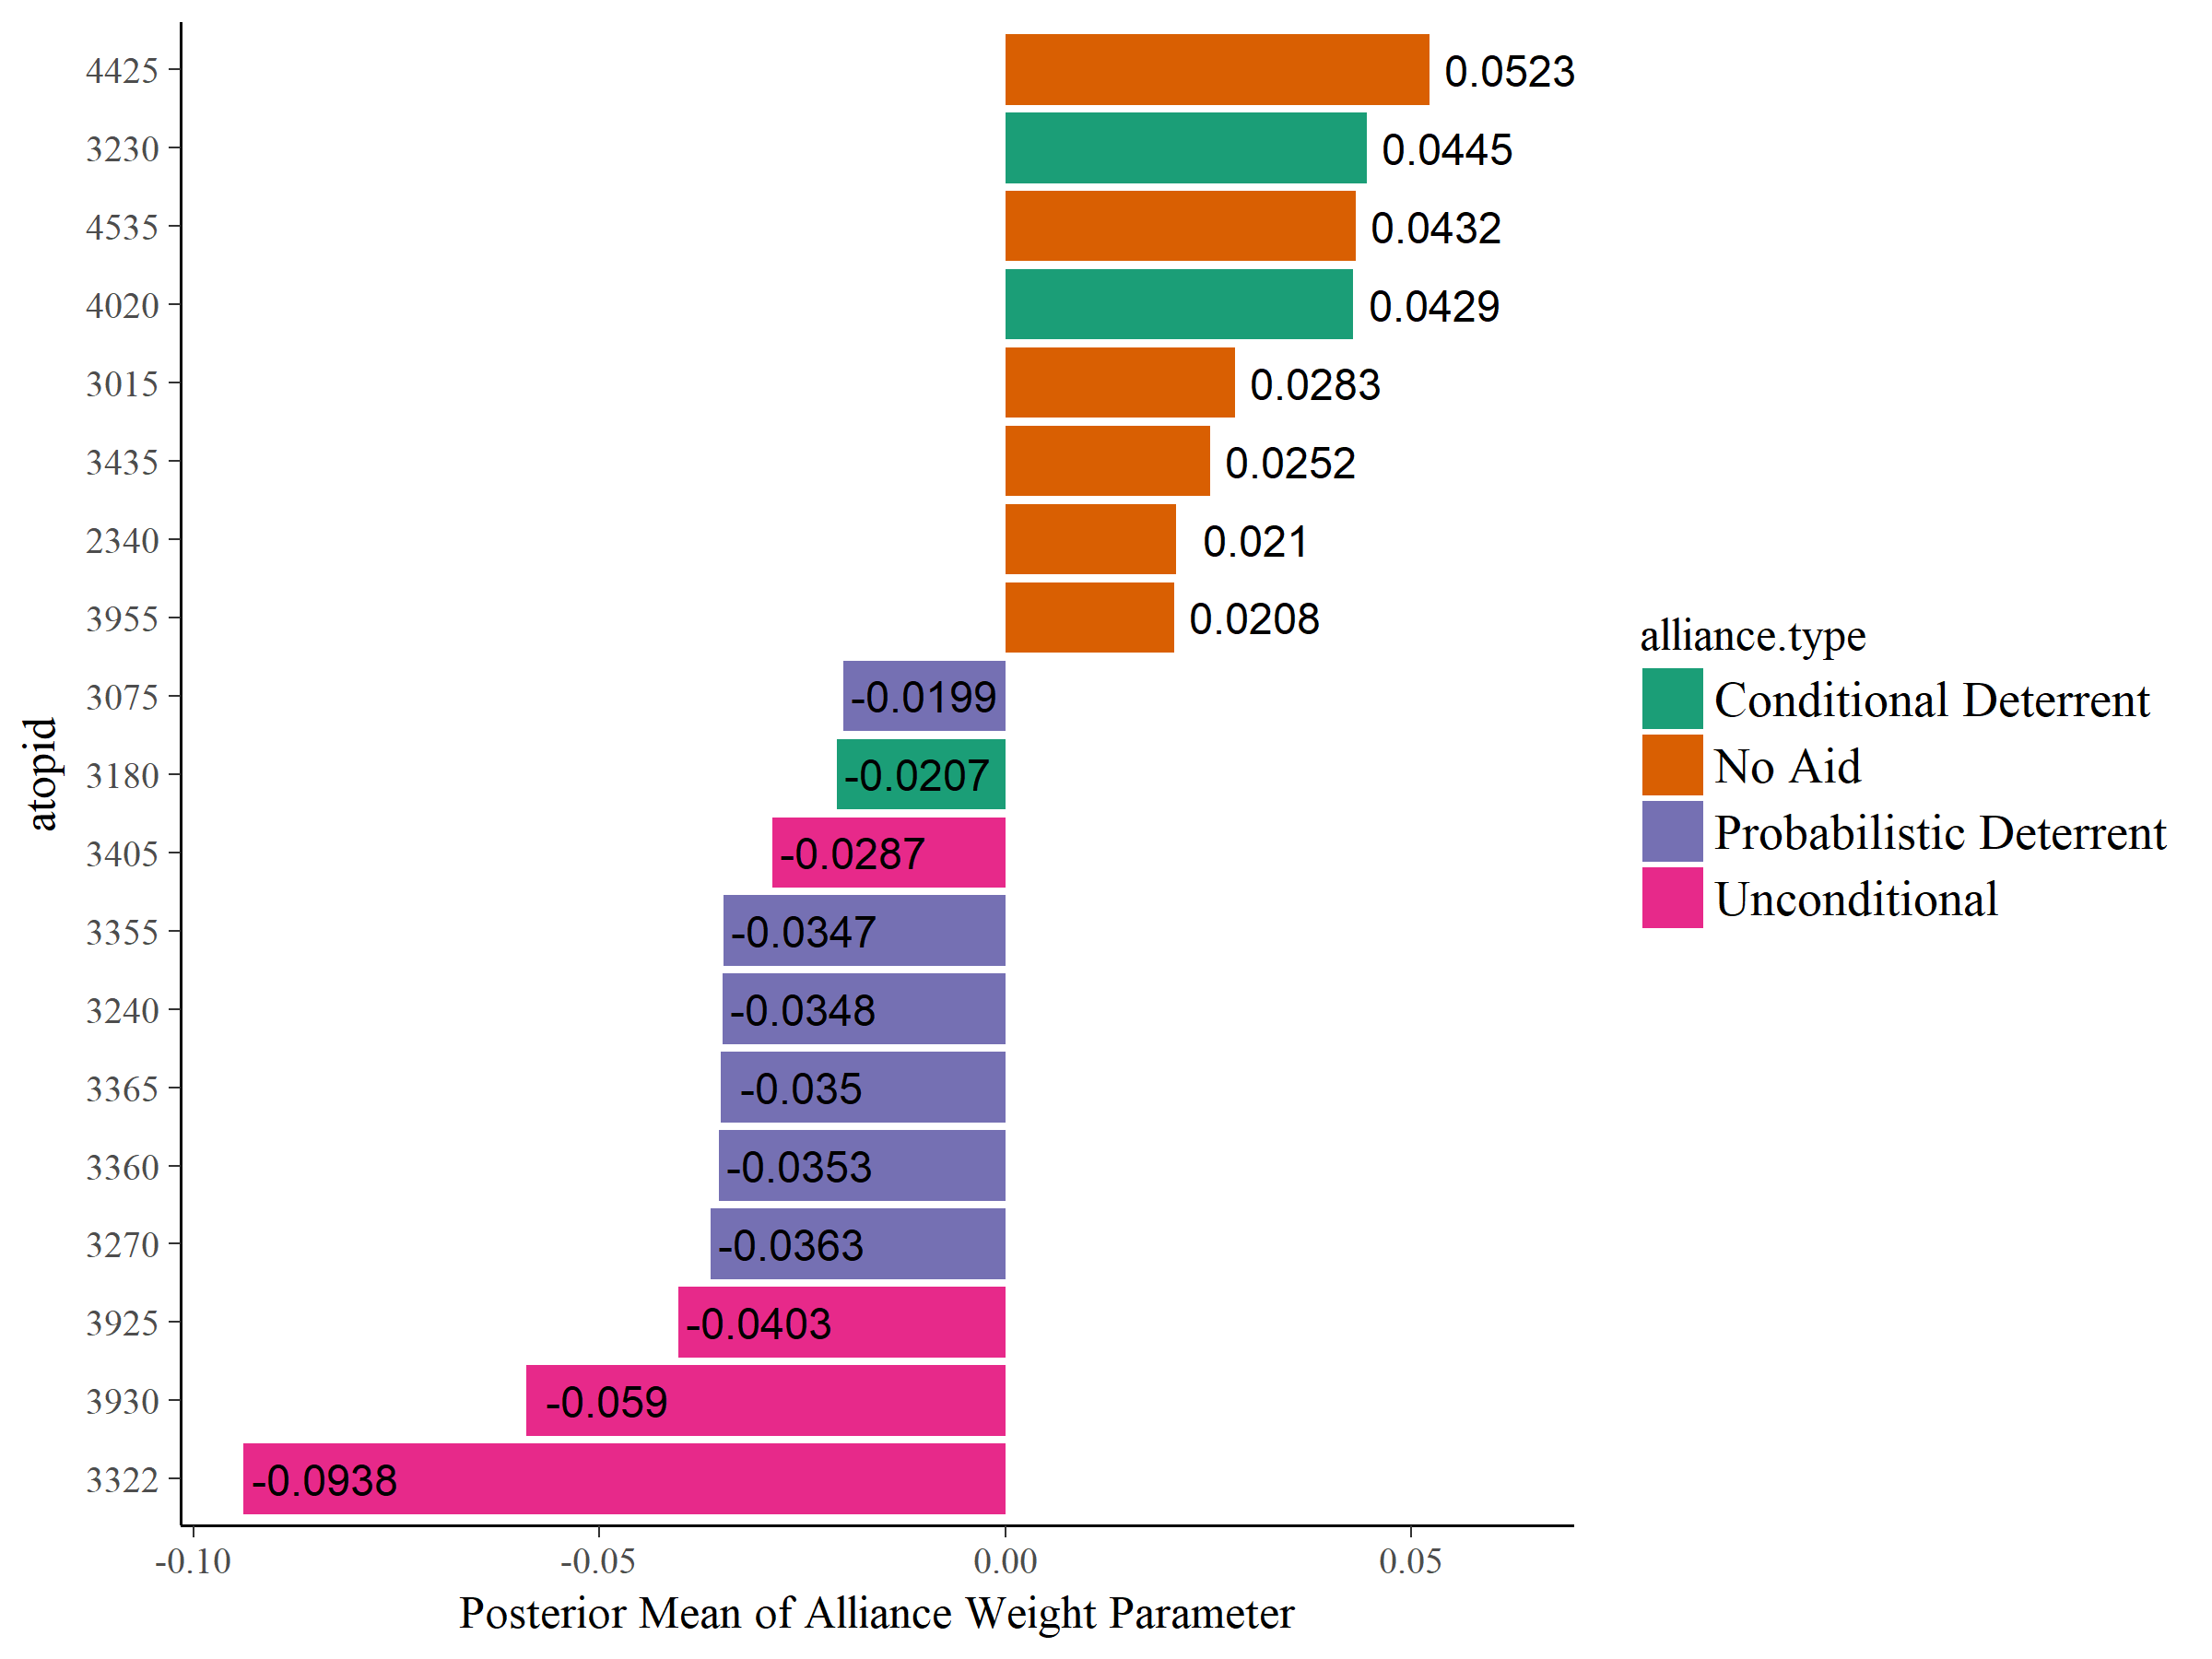
\includegraphics[width=0.95\textwidth]{non-zero alliances.png}
	\label{fig:non-zero alliances}
\end{figure}


\end{frame}

%------------------------------------------------

\begin{frame}{Violin Plot of Mean $\lambda$ for all alliances}

\begin{figure}
	\centering
		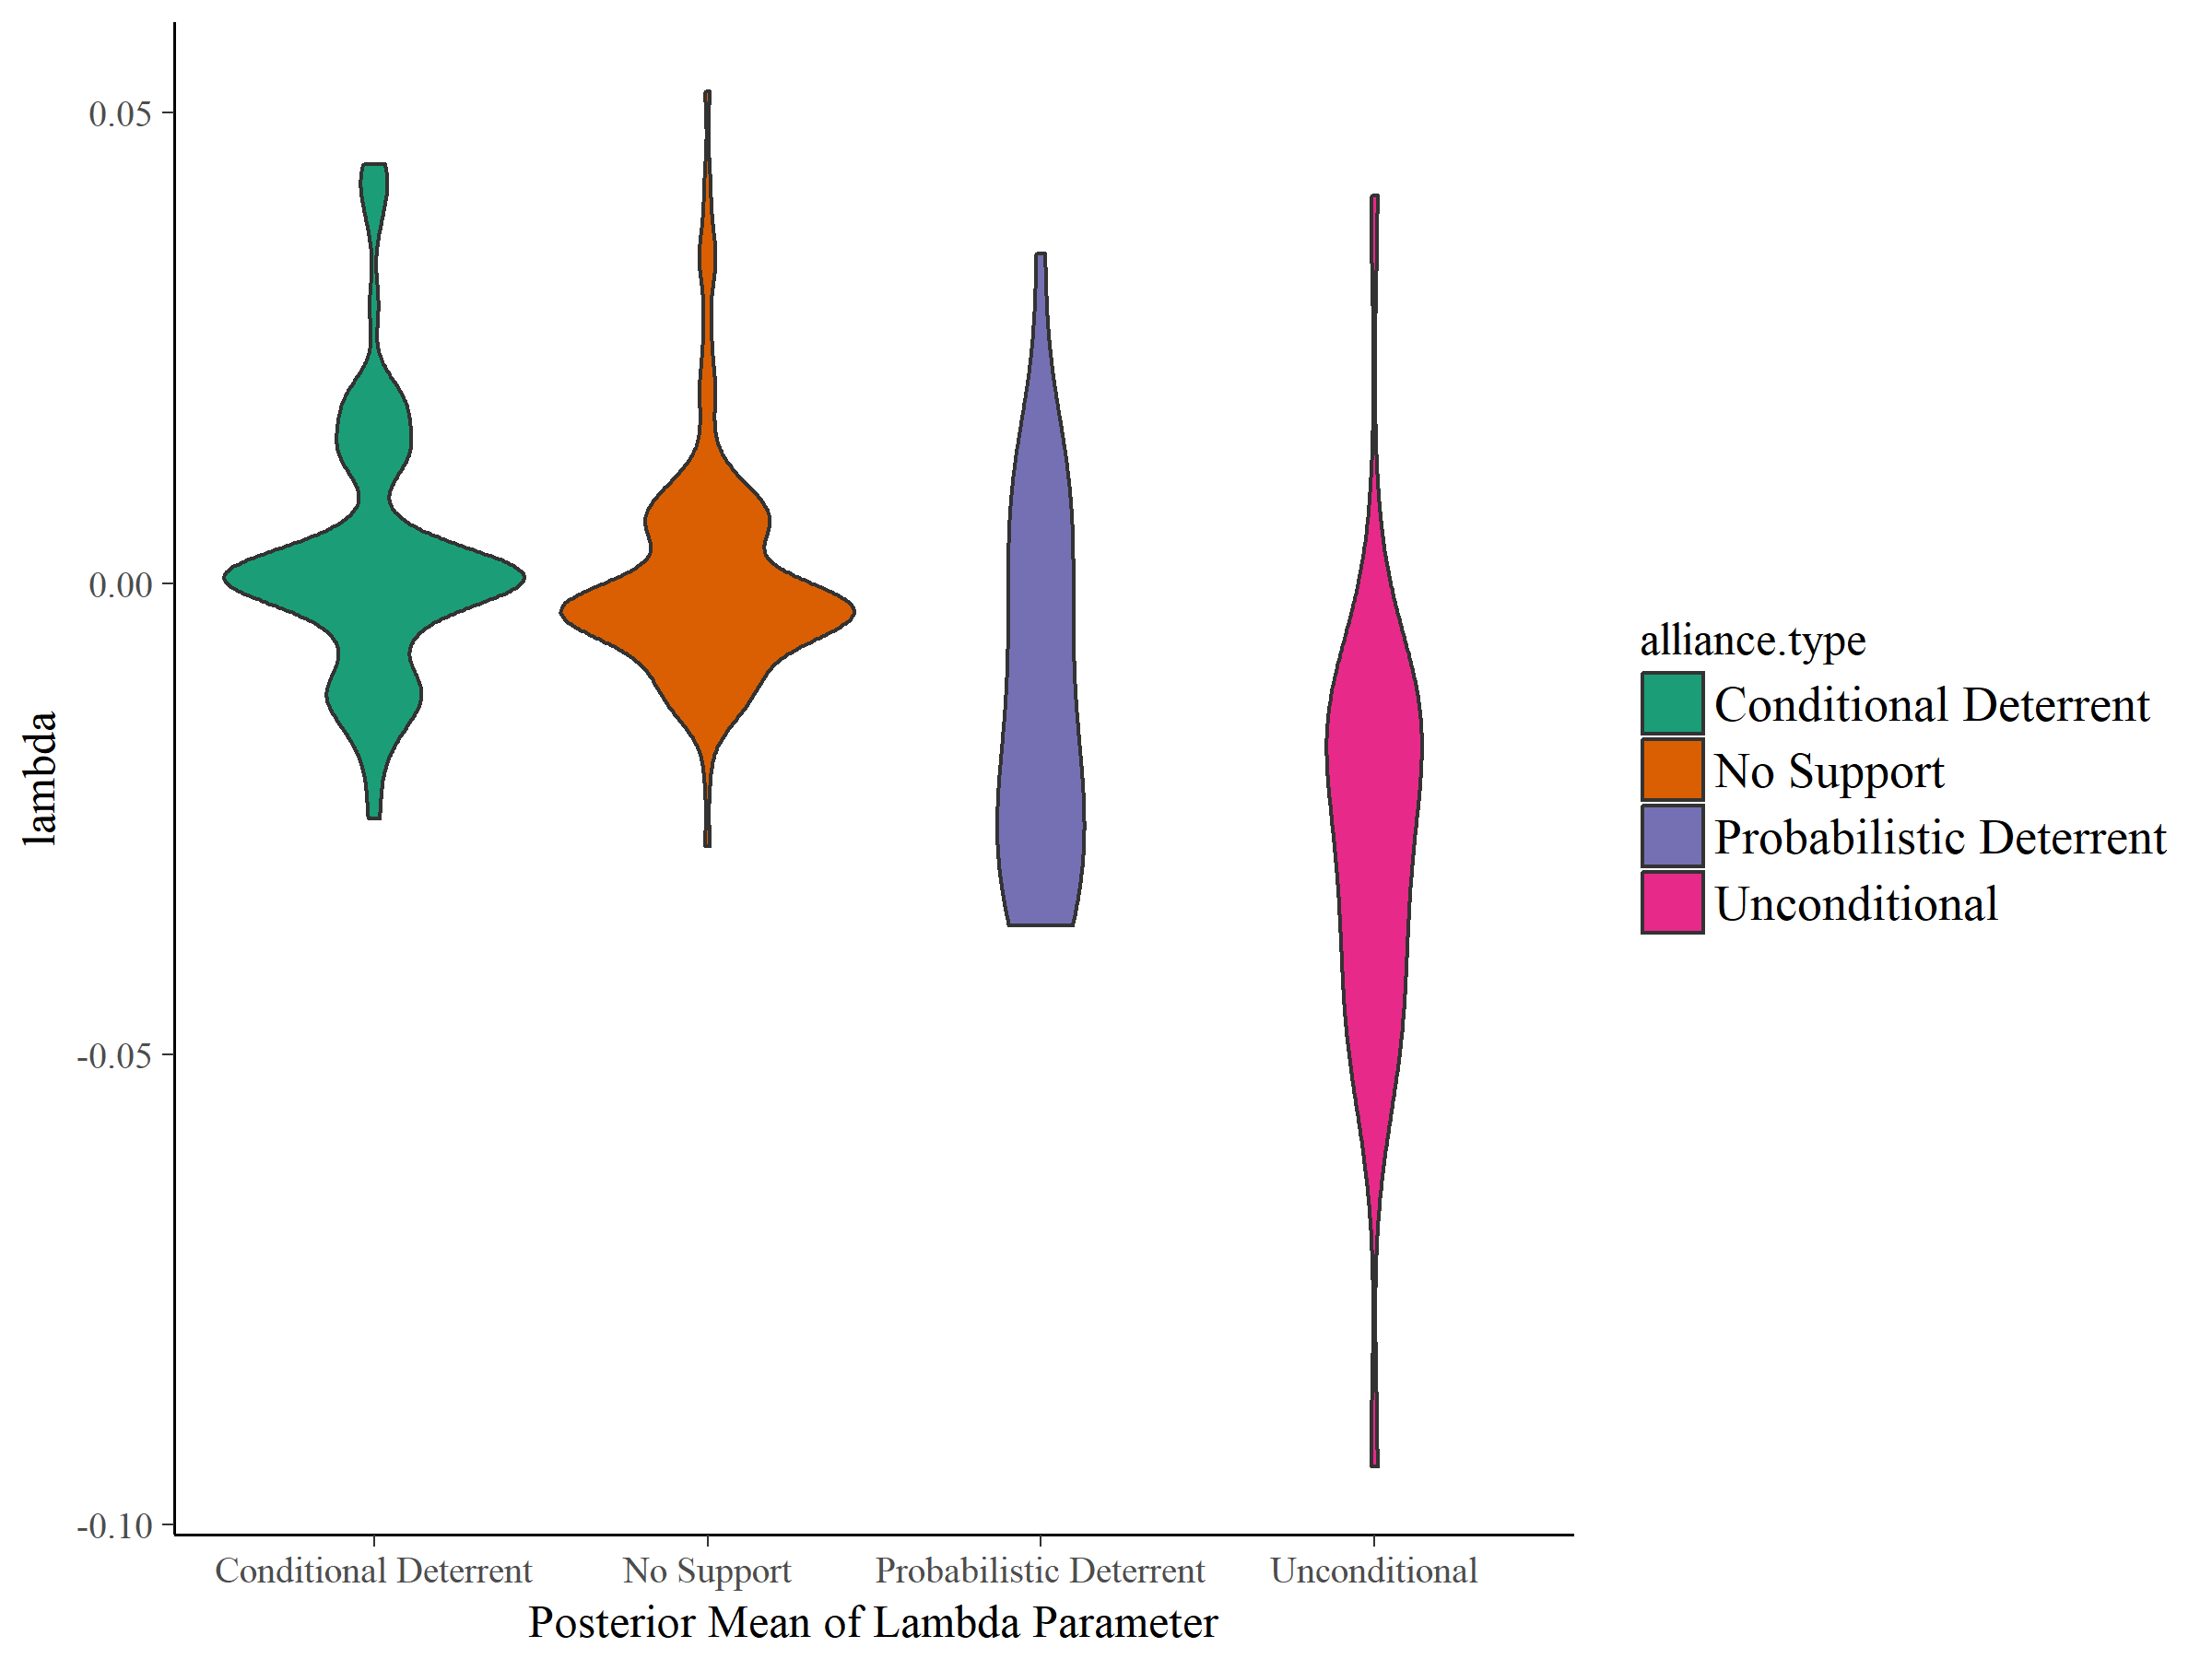
\includegraphics[width=0.95\textwidth]{C:/Users/jkalley14/Dropbox/Research/arms-allies/presentation/lambda-box-presentation-full.png}
	\label{fig:lambda-box-presentation-full}
\end{figure}


\end{frame}


%----------------------------------------------------------------------------------------

\end{document}